\documentclass[final,dvipdfmx,aspectratio=169]{beamer}

% Theme settings
\mode<presentation> {
  % \usetheme{Marburg}
  \usetheme{Metropolis}
}

%--------------- Color definitions--------------------
\definecolor{important_font}{named}{red}
\definecolor{back}{RGB}{255,255,255} % 白
% \definecolor{back}{RGB}{245,245,245} % グレー

%my-color
%\definecolor{my-color}{RGB}{0,0,0}
%\setbeamercolor{structure}{fg=my-color}

% Background color settings
%\setbeamercolor{background canvas}{bg=my-color!20}
\setbeamercolor{background canvas}{bg=white}

% Sidebar color settings
% \setbeamertemplate{sidebar canvas right}[vertical shading][top=my-color!40!black,bottom=my-color!80!black]

% Font and language settings
\usepackage{bxdpx-beamer}
\usepackage[japanese]{babel}
\usepackage{caption}
\usepackage{tikz}
\usepackage{multirow}
\usepackage{bm} 
\usepackage{color}
\usepackage{ascmac}
\usepackage{optidef}
\usepackage{subcaption}
\usepackage{tcolorbox}
\usepackage{pagecolor}
\usepackage{colortbl}
\usepackage{array}
\usepackage{xcolor}
\tcbuselibrary{breakable, skins, theorems}
\usetikzlibrary{shapes.geometric, shapes.misc, positioning}
\usetikzlibrary{decorations.markings, arrows.meta}
\usetikzlibrary{tikzmark}

% Font encoding for bookmarks
\usepackage{pxjahyper}
\usepackage{atbegshi}
\ifnum 42146=\euc"A4A2 
  \AtBeginShipoutFirst{\special{pdf:tounicode EUC-UCS2}} 
\else
  \AtBeginShipoutFirst{\special{pdf:tounicode 90ms-RKSJ-UCS2}}
\fi

% Underline with color
\makeatletter
\newlength{\chwidth}%
\newcommand{\ulinej}[1]{%
  \@tfor\ch:=#1\do%a
  {\ch%
    \settowidth{\chwidth}{\ch}%
    \hspace{-\chwidth}%
    \underline{\vphantom{あ}\phantom{\ch}}%
  }%
}%
\makeatother
\newcommand{\coloruline}[2][black]{\textcolor{#1}{\ulinej{#2}}}

% Math and font settings
\mathversion{bold}
\usefonttheme{professionalfonts}
\usefonttheme[onlymath]{serif}
\renewcommand{\familydefault}{\sfdefault}
\renewcommand{\kanjifamilydefault}{\gtdefault}

% Caption settings
\captionsetup[figure]{name=図}
\captionsetup[table]{name=表}
\setbeamertemplate{caption}[numbered]
\setbeamertemplate{footline}[frame number]

% Graphics path
\graphicspath{{img/}}

% Remove navigation symbols
\setbeamertemplate{navigation symbols}{}

% Font size settings
\setbeamerfont{caption}{size=\normalsize}
\setbeamerfont{frametitle}{size=\Large}
\setbeamerfont{block title}{size=\Large}
\setbeamerfont*{itemize/enumerate body}{size=\large}
\setbeamerfont*{itemize/enumerate subbody}{parent=itemize/enumerate body, size=\normalsize}
\setbeamerfont*{itemize/enumerate subsubbody}{parent=itemize/enumerate subbody, size=\normalsize}
\setbeamerfont{section in toc}{size=\small} % セクションのフォントサイズを小さく
\setbeamerfont{subsection in toc}{size=\scriptsize} % サブセクションのフォントサイズをさらに小さく


% Frame title color settings
% \setbeamercolor{frametitle}{fg=white,bg=my-color!40!black}

% Block environment settings
\setbeamercolor{block body}{bg=back}
\setbeamercolor{bibliography entry author}{fg=black}
\setbeamercolor{bibliography entry journal}{fg=black}
\setbeamercolor{bibliography entry note}{fg=black}
\setbeamercolor{bibliography entry publisher}{fg=black}

% Bibliography formatting
\beamertemplatetextbibitems


\begin{document}
\title[Swaq]{\color{black} \LARGE SWAQ}
\subtitle[ちょっと強いQAS]{特定の問題にちょっと強くなった量子アニーリングシミュレーター}
\author[岡田颯斗]{岡田颯斗}
\institute[大阪府立四條畷高等学校]{大阪府立四條畷高等学校}
\date{}
\begin{frame}{}
\titlepage
\end{frame}
\large

\begin{frame}
  \frametitle{目次}
  \tableofcontents
\end{frame}

%add here

\section{自己紹介}
\begin{frame}
  \frametitle{どうもこんにちは}
  \begin{itemize}
      \item 名前:岡田颯斗(高校3年生)
      \item 趣味・興味:
      \begin{itemize}
          \item 競技数学
          \item 量子コンピュータ
      \end{itemize}
  \end{itemize}
\end{frame}

\section{前提}
\begin{frame}
  \frametitle{量子アニーリングは組合せ最適化問題を解く手段の一つ}
  よく扱われる問題の例:\\
  \vspace{10mm}
  \begin{columns}
    \begin{column}{0.45\textwidth}
      \textbf{彩色問題}
      \begin{itemize}
          \item 隣り合う場所は異なる色で塗分ける
      \end{itemize}
    \end{column}

    \begin{column}{0.45\textwidth}
      \textbf{巡回セールスマン問題}
      \begin{itemize}
          \item 複数の街を最短経路ですべて訪れる
      \end{itemize}
    \end{column}
  \end{columns}
  \vspace{5mm}
\end{frame}

\begin{frame}
  \frametitle{彩色問題}
  %4×4のほう
  彩色問題:リンク\\
\end{frame}


\begin{frame}
  \frametitle{だがしかし}

  {\Large  量子アニーリングは組合せ最適化問題を解く手段の一つ}
  \vspace{5mm}

  \begin{columns}
    \begin{column}{0.45\textwidth}
      \textbf{彩色問題}
      \begin{itemize}
          \item 隣り合う場所は異なる色で塗分ける
      \end{itemize}
    \end{column}

    \begin{column}{0.45\textwidth}
      \textbf{巡回セールスマン問題}
      \begin{itemize}
          \item 複数の街を最短経路ですべて訪れる
      \end{itemize}
    \end{column}
  \end{columns}
  \vspace{10mm}
  \pause{\color{important_font}しかし、量子アニーリングは最適化問題を効率よく解けるかというと...}
\end{frame}

\section{背景}
\begin{frame}
  \frametitle{量子アニーリングはm個の中からn個選ぶのが苦手}
  
  なぜなら...\\
  \begin{itemize}
    \item 制約がペナルティ項として目的関数につけられてしまう
    \item すると問題が非本質な方向へ最適化される
  \end{itemize}

  \vspace{5mm}

  \only<1>{\[
    \begin{aligned}
        &\text{minimize} \quad H_{object} \\
        &\text{subject to} \quad H_{constraint} = c
    \end{aligned}
  \]}

  \only<2>{\[
    \begin{aligned}
        &\text{minimize} \quad H_{object} + \underbrace{(H_{constraint} - c)^2}_{H_{penalty}} \\
    \end{aligned}
  \]}

\end{frame}

\subsection{問題例}
\begin{frame}
  \frametitle{式で見ると}
    \begin{columns}[T]
      \begin{column}{0.47\textwidth}
        {\large 彩色問題}
        \footnotesize{
        \[
          \begin{aligned}
              &\text{minimize} \quad \sum_{i,j\in Adj}\sum_{k\in color}q_{i,k}q_{j,k} \\
              &\text{subject to} \quad \sum_{i\in vertics}q_{i,k} = 1 
          \end{aligned}
        \]\\
        \begin{center}
          ${\large \downarrow}$
        \end{center}
        \begin{tcolorbox}[top=0mm, left=0mm, right=0mm, bottom=0mm]
        \[
          \begin{aligned}
              \text{minimize} \quad \sum_{i,j\in Adj}\sum_{k\in color}q_{i,k}q_{j,k}\\
               + \sum_{k\in color}(\sum_{i\in Adj}q_{i,k}-1)^2\\
          \end{aligned}
        \]  
        \end{tcolorbox}
        }
      \end{column}  

      \begin{column}{0.55\textwidth}
        {\large 巡回セールスマン問題}
        \footnotesize{
        \[
          \begin{aligned}
              &\text{minimize} \quad  & & \sum_{i,j\in C}\sum_{k = 0}^n w_{i,j}q_{i,k}q_{j,k+1} \\
              &\text{subject to} \quad& & \sum_{i\in C}q_{i,k} = 1 \\
              &                       & & \sum_{k = 0}^n q_{i,k} = 1
          \end{aligned}
        \]\\
        \begin{center}
          ${\large \downarrow}$
        \end{center}
        \begin{tcolorbox}[top=0mm, left=1mm, right=0mm, bottom=0mm]
        \[
          \begin{aligned}
              &\text{minimize} \quad \sum_{i,j\in C}\sum_{k = 0}^n w_{i,j}q_{i,k}q_{j,k+1}\\
               &+ \sum_{k=0}^n(\sum_{i\in C}q_{i,k}-1)^2+\sum_{i\in C}(\sum_{k=0}^nq_{i,k}-1)^2\\
          \end{aligned}
        \]  
        \end{tcolorbox}
        }
      \end{column}  
    \end{columns}
\end{frame}

\begin{frame}
  \frametitle{つまり}

  {\Large   量子アニーリングは組合せ最適化問題を解く手段の一つ}
  \vspace{5mm}

  \begin{columns}
    \begin{column}{0.45\textwidth}
      \textbf{彩色問題}
      \begin{itemize}
          \item 隣り合う場所は異なる色で塗分ける
          \item {\color{important_font}各地点はちょうど一色で塗られる}
      \end{itemize}
    \end{column}

    \begin{column}{0.45\textwidth}
      \textbf{巡回セールスマン問題}
      \begin{itemize}
          \item 複数の街を最短経路ですべて訪れる
          \item {\color{important_font}各時間に訪れることのできるサイトはちょうど1か所}
          \item {\color{important_font}各地点ちょうど1回訪れる}
      \end{itemize}
    \end{column}
  \end{columns}
  \vspace{5mm}
  \pause{これらの制約を常に満たすように解を遷移させていけば効率が上がりそう}
\end{frame}

\section{デモ}
\begin{frame}
  \frametitle{彩色問題(再)}
  エネルギーが下がっていく様子を付けた20×20の彩色問題の動画
\end{frame}

\section{手法}
\begin{frame}
  \frametitle{簡単な例:彩色問題}
  \begin{table}
    \centering
    \begin{tabular}{c|c c c c c}
        \textbf{$q_{i,j}$} & \textbf{場所1} & \textbf{場所2} & \textbf{場所3} & \textbf{場所4} & \textbf{場所5} \\
        \hline
        \textbf{色1} &{\cellcolor{blue!50}} 0 & 0                                         &{\cellcolor{blue!50}} \color{orange}1 & 0 &{\cellcolor{blue!50}} 0  \\
        \textbf{色2} &{\cellcolor{blue!50}} \color{orange}1 & 0\only<2>{\tikzmark{A}\cellcolor{yellow}} &{\cellcolor{blue!50}} 0 & \color{orange}1 &{\cellcolor{blue!50}} 0  \\
        \textbf{色3} &{\cellcolor{blue!50}} 0 & 0                                         &{\cellcolor{blue!50}} 0 & 0 &{\cellcolor{blue!50}} \color{orange}1  \\
        \textbf{色4} &{\cellcolor{blue!50}} 0 & \color{orange}1\only<2>{\tikzmark{B}\cellcolor{yellow}} &{\cellcolor{blue!50}} 0 & 0 &{\cellcolor{blue!50}} 0  \\
    \end{tabular}
  \end{table}
  \hspace{4.4cm}$\uparrow$\hspace{1.3cm}$\uparrow$\hspace{1.3cm}$\uparrow$\hspace{1.3cm}$\uparrow$\hspace{1.3cm}$\uparrow$\\
  \centering{各列1はちょうど1つ}
  \tikzset{arrow style/.style={->, thick, draw=black, rounded corners, shorten >=5pt, shorten <=5pt, line width=1.5pt}}
  \begin{tikzpicture}[remember picture,overlay,baseline=0pt] 
    \only<2>{
    \draw[arrow style, bend left=-60] ([shift={(-0.5ex,0)}]pic cs:A) to ([shift={(-0.5ex,0)}]pic cs:B);
    \draw[arrow style, bend left=-60] ([shift={(-0.5ex,0)}]pic cs:B) to ([shift={(-0.5ex,0)}]pic cs:A);}
  \end{tikzpicture}

\end{frame}

\begin{frame}
  \frametitle{その次くらいに簡単な例:巡回セールスマン}

  \begin{table}
    \centering
    \begin{tabular}{c|c c c c c}
        \textbf{$q_{i,j}$} & \textbf{場所1} & \textbf{場所2} & \textbf{場所3} & \textbf{場所4} & \textbf{場所5} \\
        \hline
        \textbf{順番1} &{\cellcolor{blue!50}} 0 & 0 &{\cellcolor{blue!50}} \color{orange}1 & 0 &{\cellcolor{blue!50}} 0  \\
        \textbf{順番2} &{\cellcolor{blue!50}}\color{orange} 1 & 0 &{\cellcolor{blue!50}} 0 & 0 &{\cellcolor{blue!50}} 0  \\
        \textbf{順番3} &{\cellcolor{blue!50}} 0 & 0 &{\cellcolor{blue!50}} 0 & 0 &{\cellcolor{blue!50}} \color{orange}1  \\
        \textbf{順番4} &{\cellcolor{blue!50}} 0 & 0 &{\cellcolor{blue!50}} 0 & \color{orange}1 &{\cellcolor{blue!50}} 0  \\
        \textbf{順番5} &{\cellcolor{blue!50}} 0 & \color{orange}1 &{\cellcolor{blue!50}} 0 & 0 &{\cellcolor{blue!50}} 0  \\
    \end{tabular}
  \end{table}
  \hspace{4.65cm}$\uparrow$\hspace{1.3cm}$\uparrow$\hspace{1.3cm}$\uparrow$\hspace{1.3cm}$\uparrow$\hspace{1.3cm}$\uparrow$\\
  \centering{各列1はちょうど1つ}
\end{frame}

\setcounter{framenumber}{11}
\begin{frame}
  \frametitle{その次くらいに簡単な例:巡回セールスマン}
  \begin{columns}
    \begin{column}{0.9\linewidth}
      \begin{table}
        \centering
        \begin{tabular}{c|c c c c c}
            \textbf{$q_{i,j}$} & \textbf{場所1} & \textbf{場所2} & \textbf{場所3} & \textbf{場所4} & \textbf{場所5} \\
            \hline
            \rowcolor{blue!50}
            \textbf{順番1} & 0 & 0 & \color{orange}1 & 0 & 0  \\
            \textbf{順番2} & \color{orange}1 & 0 & 0 & 0 & 0  \\
            \rowcolor{blue!50}
            \textbf{順番3} & 0 & 0 & 0 & 0 & \color{orange}1  \\
            \textbf{順番4} & 0 & 0 & 0 & \color{orange}1 & 0  \\
            \rowcolor{blue!50}
            \textbf{順番5} & 0 & \color{orange}1 & 0 & 0 & 0  \\
        \end{tabular}
      \end{table}        
    \end{column}
    \begin{column}{0.3\linewidth}
      \vspace{3mm}\\
      $\leftarrow$  各\\
      $\leftarrow$  行\\
      $\leftarrow$  も\\
      $\leftarrow$  同\\
      $\leftarrow$  様
    \end{column}
  \end{columns}
  

\end{frame}

\setcounter{framenumber}{11}
\begin{frame}
  \frametitle{その次くらいに簡単な例:巡回セールスマン}

  \begin{table}
    \centering
    \begin{tabular}{c|c c c c c}
        \textbf{$q_{i,j}$} & \textbf{場所1} & \textbf{場所2} & \textbf{場所3} & \textbf{場所4} & \textbf{場所5} \\
        \hline
        \textbf{順番1} & 0                                         & 0                         & 1 & 0 & 0  \\
        \textbf{順番2} & 1{\tikzmark{a}\cellcolor{yellow}} & 0{\tikzmark{b}\cellcolor{yellow}} & 0 & 0 & 0  \\
        \textbf{順番3} & 0                                         & 0                         & 0 & 0 & 1  \\
        \textbf{順番4} & 0                                         & 0                         & 0 & 1 & 0  \\
        \textbf{順番5} & 0{\tikzmark{c}\cellcolor{yellow}} & 1{\tikzmark{d}\cellcolor{yellow}} & 0 & 0 & 0  \\
    \end{tabular}
  \end{table}
  \tikzset{arrow style/.style={->, thick, draw=black, rounded corners, shorten >=5pt, shorten <=5pt, line width=1.5pt}}
  \begin{tikzpicture}[remember picture,overlay,baseline=0pt] 
    {
    \draw[arrow style, bend left=-60] ([shift={(-0.5ex,0)}]pic cs:a) to ([shift={(-0.5ex,0)}]pic cs:c);
    \draw[arrow style, bend left=-60] ([shift={(-0.5ex,0)}]pic cs:b) to ([shift={(-0.5ex,0)}]pic cs:d);
    \draw[arrow style, bend left=-60] ([shift={(-0.5ex,0)}]pic cs:c) to ([shift={(-0.5ex,0)}]pic cs:a);
    \draw[arrow style, bend left=-60] ([shift={(-0.5ex,0)}]pic cs:d) to ([shift={(-0.5ex,0)}]pic cs:b);}
  \end{tikzpicture}

\end{frame}

\section{比較}
\begin{frame}
  \frametitle{比較}
  \begin{figure}
    \begin{columns}
      \begin{column}{0.47\linewidth}
        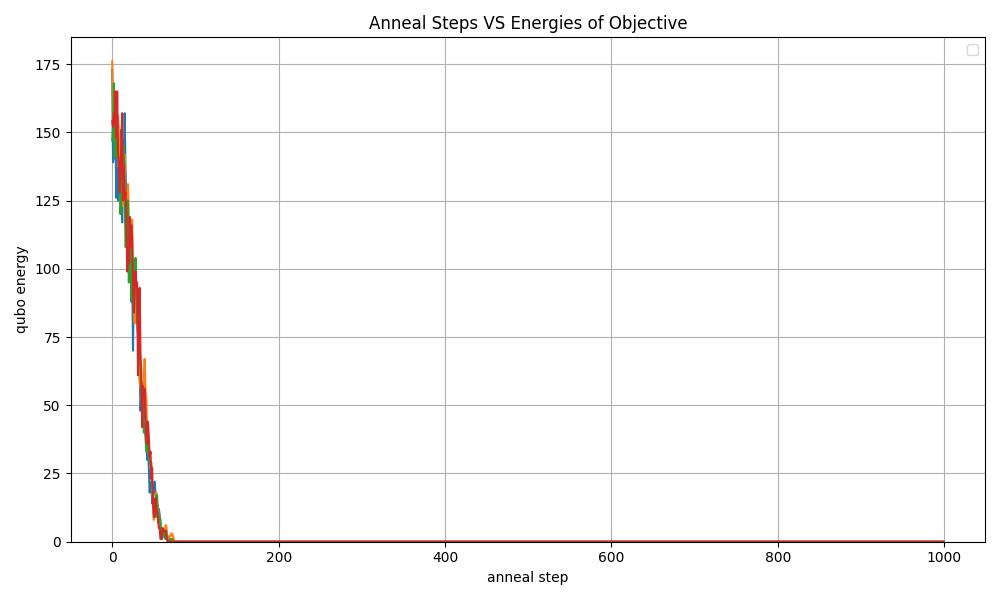
\includegraphics[width=1\linewidth]{data/GC_ene.png}
        \caption{Swap basedのQAS (lowest = 0)}        
      \end{column}
      \begin{column}{0.47\linewidth}
        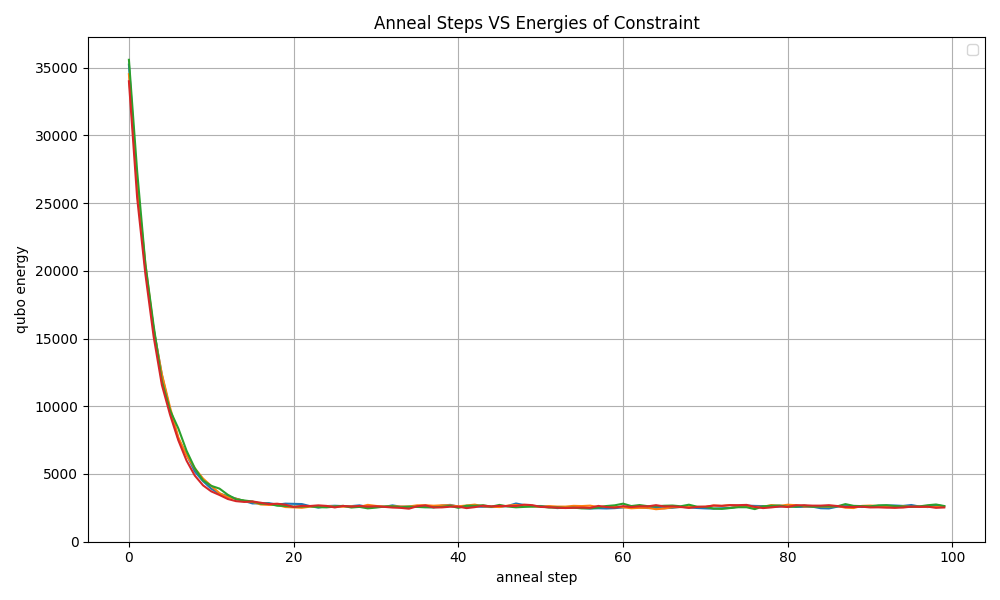
\includegraphics[width=1\linewidth]{data/GC_onehot_ene.png}
        \caption{普通のQAS (lowest = 2630)}
      \end{column}
    \end{columns}
  \end{figure}
  ※縦軸の目盛りが異なることに注意
\end{frame}

\section{展望}
\begin{frame}
  \frametitle{一般化をしたい}
  \begin{figure}
    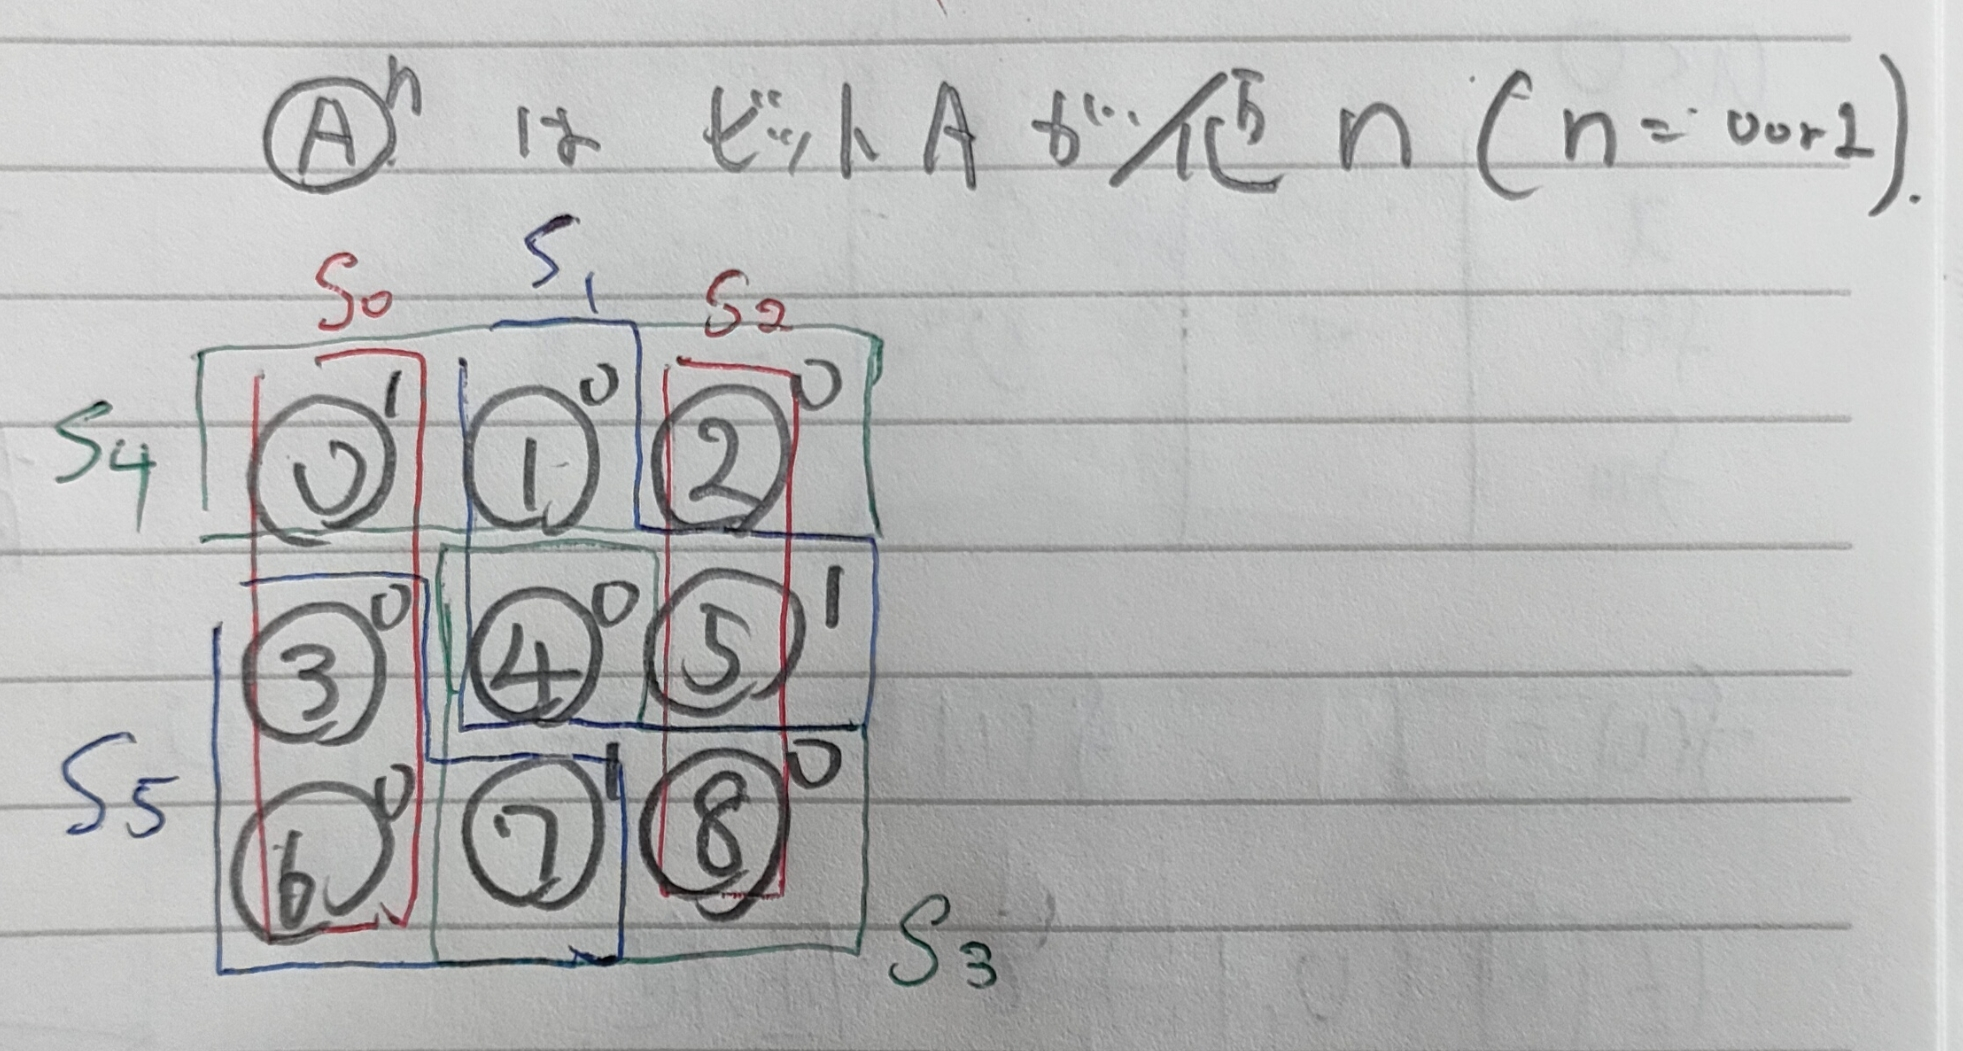
\includegraphics[width=0.47\linewidth]{data/rakugaki1.jpg}
    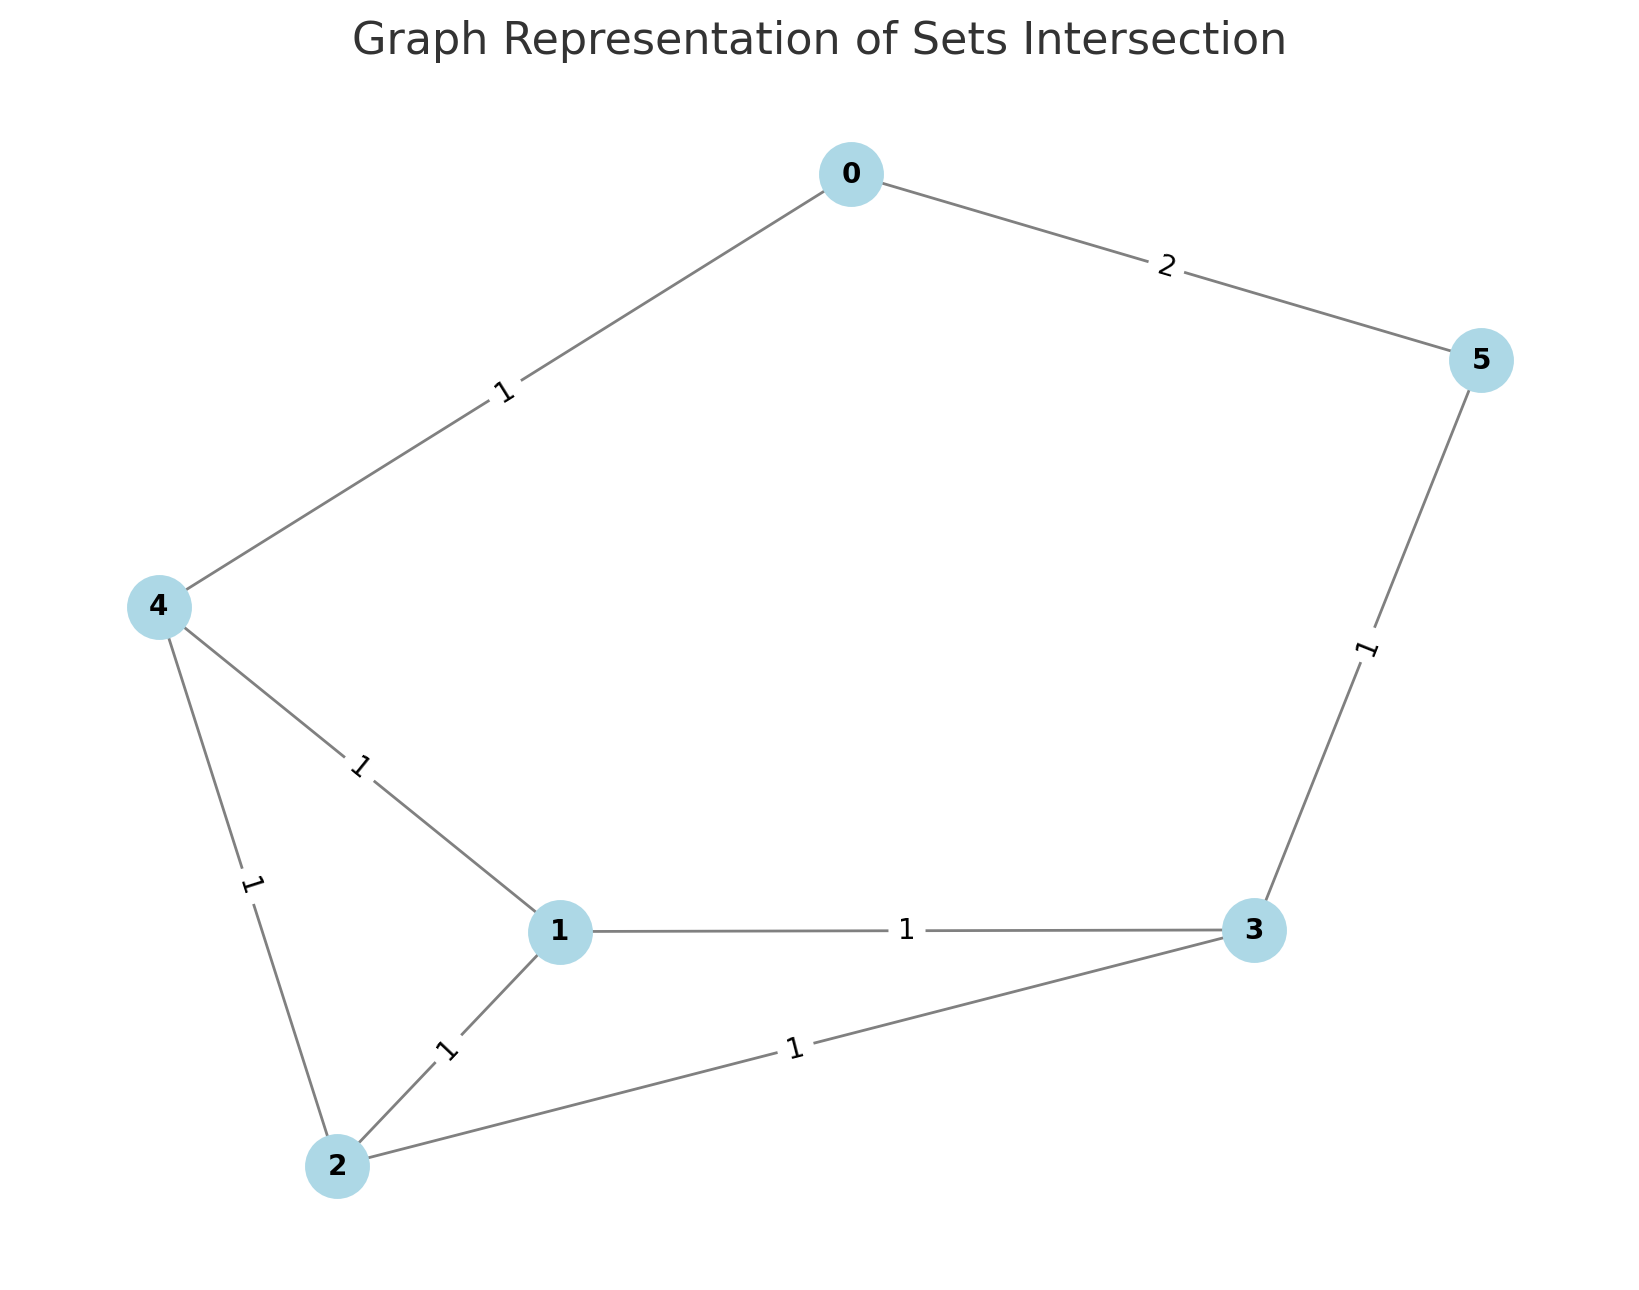
\includegraphics[width=0.47\linewidth]{data/graph1.png}
  \end{figure}
  こんな感じの図をきれいにつくる
\end{frame}


\begin{frame}[t]{参考文献}
  \footnotesize

  \bibliographystyle{junsrt}
  \bibliography{bibliography.bib}
\end{frame}




\end{document}
